\lstinputlisting[language=bash,basicstyle=\small]{python_codes/fieldstone_46/keywords}

\begin{center}
Code at \url{https://github.com/cedrict/fieldstone/tree/master/python_codes/fieldstone_46}
\end{center}

\par\noindent\rule{\textwidth}{0.4pt}
%%%%%%%%%%%%%%%%%%%%%%%%%%%%%%%%%%%%%%%%%%%%%%%%%%%%%%%%%%%%%%%%%%%%%%%%%%%%%%%%%%%%%%%%%%%%%

This stone showcases the Crouzeix-Raviart element (see Section~\ref{sec:crouzeix-raviart})
used to solve the analytical problem "Donea \& Huerta" (see Section~\ref{mms1}).

Out of convenience the pressure is set to zero at location $(x,y)=(1,1)$, so that the 
analytical solution is now $p(x,y)=x(1-x)$. 

\begin{center}
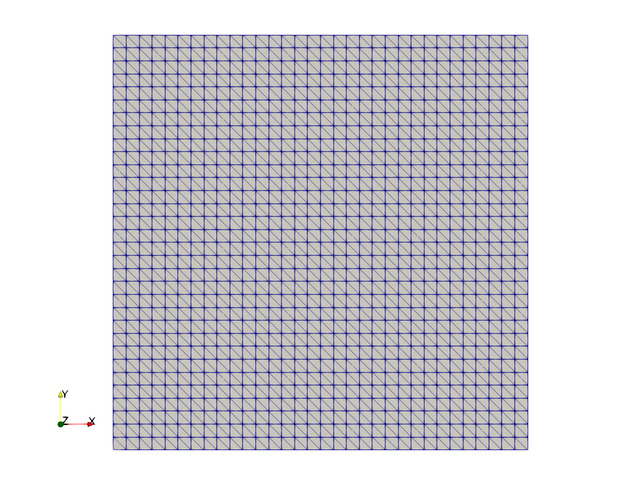
\includegraphics[width=5cm]{python_codes/fieldstone_46/results/grid}
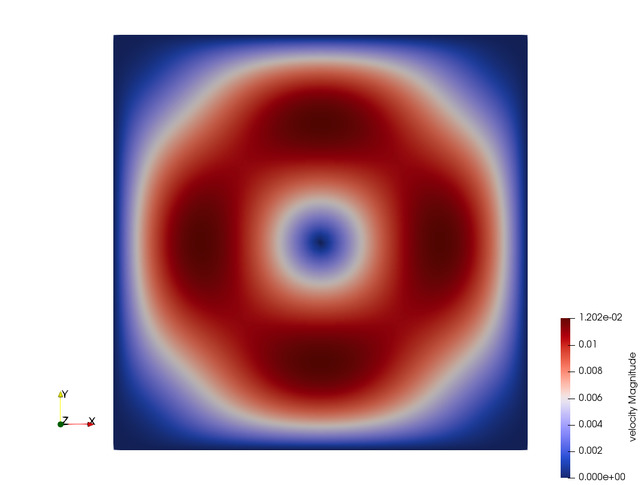
\includegraphics[width=5cm]{python_codes/fieldstone_46/results/vel}
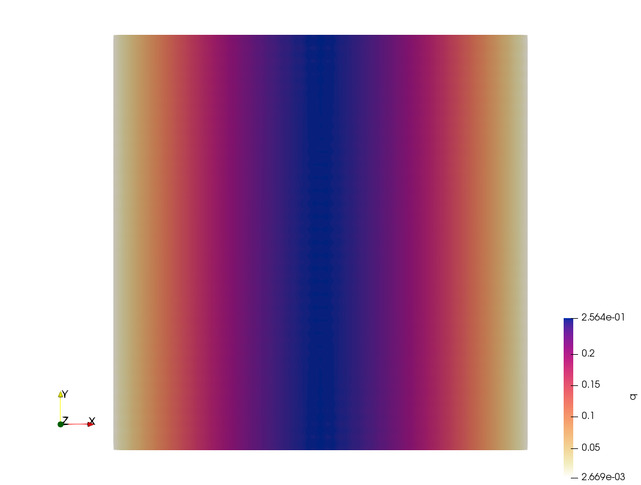
\includegraphics[width=5cm]{python_codes/fieldstone_46/results/press}\\
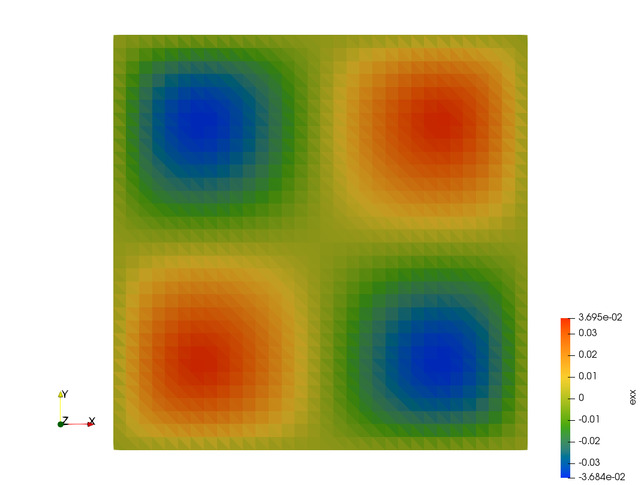
\includegraphics[width=5cm]{python_codes/fieldstone_46/results/exx}
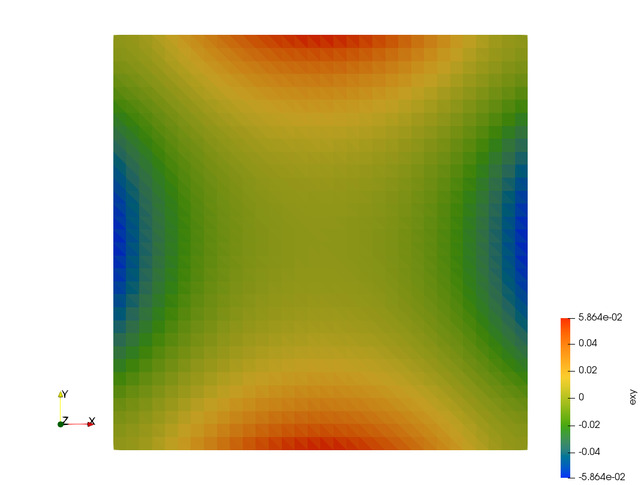
\includegraphics[width=5cm]{python_codes/fieldstone_46/results/exy}
\end{center}

\begin{center}
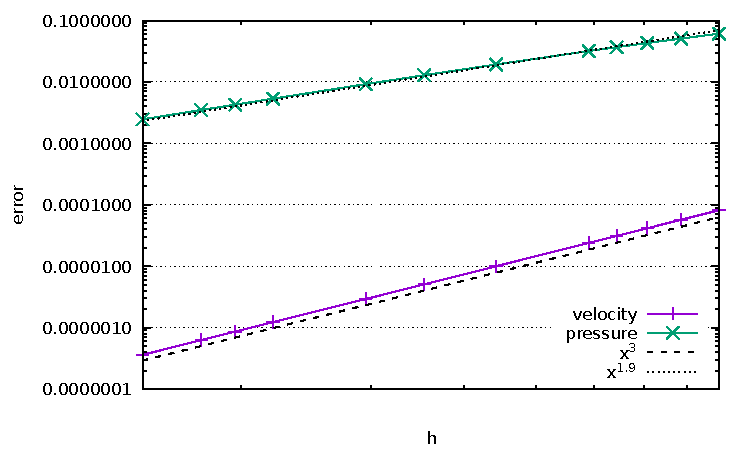
\includegraphics[width=14cm]{python_codes/fieldstone_46/results/errors.pdf}
\end{center}

I seem to just not quite obtain a quadratic convergence for pressure. Could it come 
from the p b c ?
